\section{Variables y preparación de datos}
\label{sec:datos}

Las \emph{fibras} son los elementos alargados de la malla y los \emph{pivotes}, sus conectores deformables. Una familia comparte la cantidad de celdas en Y ($4$, $5$ o $6$). En los ensayos de tracción con carga--descarga, la \emph{carga de primera falla} identifica la fuerza del primer evento de rotura, anterior o coincidente con la rotura terminal \cite{venditti2025}.

\begin{table}[htbp]
\centering\small\setstretch{1.0}
\caption{Diccionario de variables del análisis. Las salidas posteriores se excluyen de los predictores.}
\label{tab:diccionario}
\begin{tabularx}{\linewidth}{@{}p{3.3cm}lYl@{}}
\toprule
Variable & Unidad & Significado & Rol \\
\midrule
Celdas en Y & conteo & Celdas de la malla en esa dirección; define familia. & Entrada \\
Altura de fibra & mm & Altura de la sección rectangular, $h$. & Entrada \\
Ancho de fibra & mm & Base de la sección rectangular, $b$. & Entrada \\
Longitud de fibras & mm & Longitud total declarada de fibras. & Entrada \\
Volumen de fibras & mm$^3$ & Volumen declarado del conjunto de fibras, $V_f$. & Entrada \\
Altura de pivote & mm & Altura del conector entre fibras. & Entrada \\
Radio de pivote & mm & Radio del conector; constante en los datos. & Entrada \\
Cantidad de pivotes & conteo & Conectores de la estructura. & Entrada \\
Volumen de pivotes & mm$^3$ & Volumen declarado de los conectores, $V_p$. & Entrada \\
Volumen CAD & mm$^3$ & Volumen del espécimen en CAD, distinto de $V_f+V_p$. & Entrada \\
\midrule
Carga de primera falla & N & Fuerza asociada a la primera rotura identificada. & Salida objetivo \\
Carga terminal & N & Fuerza terminal reportada; no necesariamente máxima. & Salida \\
Desplazamiento máximo & mm & Máximo desplazamiento registrado en el resumen. & Salida \\
Desplazamientos residuales & mm & Desplazamiento que permanece tras descargar cada ciclo. & Salida \\
Energía disipada & mJ & Energía tabulada por ciclo de carga--descarga. & Salida \\
Energía de fractura & mJ & Energía tabulada asociada a un evento de rotura. & Salida \\
\midrule
Identificador del caso & --- & Vincula geometría y respuestas; no entra al modelo. & Control \\
\bottomrule
\end{tabularx}
\par\smallskip\small Fuente: diccionario del repositorio y variables de los cuadernos 01--03. Los valores son dimensiones declaradas, no tolerancias de fabricación medidas.
\end{table}


La predicción precede al ensayo: cargas posteriores, desplazamientos, energías e identificadores quedan excluidos de las entradas, aunque presenten correlación con el objetivo.

\subsection{Curaduría: qué se revisó y qué se modificó}
El notebook 01 convierte las asignaciones MATLAB en tablas, valida tipos y conserva ausentes. Se comprobó la equivalencia valor a valor; la curaduría normalizó la representación sin generar geometrías ni fuerzas (Tabla~\ref{tab:curaduria}).

\begin{table}[htbp]
\centering\small\setstretch{1.0}
\caption{Curaduría aplicada y efecto sobre el análisis.}
\label{tab:curaduria}
\begin{tabularx}{\linewidth}{@{}YYY@{}}
\toprule
Control & Resultado observado & Tratamiento aplicado \\
\midrule
Extracción y tipos & Las asignaciones numéricas y sus nulos coinciden con las tablas extraídas. & Lectura literal sin ejecutar MATLAB; conversión numérica y conservación de identificadores. \\
\addlinespace
Valores faltantes & Geometría completa; ausencia conjunta de respuestas en una entrada de la fuente. & No inventar el objetivo; conservar la geometría y excluir de supervisión la respuesta ausente. \\
\addlinespace
Dominios & Dimensiones positivas, conteos enteros y carga objetivo positiva. & Validar unidades y dominios; ninguna corrección de valores por estos controles. \\
\addlinespace
Repetición & Sin filas exactamente duplicadas; coincidencias de factores con otras medidas distintas. & Conservar sin promediar; reunir configuraciones relacionadas durante validación. \\
\addlinespace
Consistencia y extremos & Radio constante; discrepancias de volúmenes frente a formas ideales; energías iniciales negativas. & Filtrar el radio en entrenamiento; conservar signos y casos señalados; no corregir mediante fórmulas ideales. \\
\addlinespace
Respuestas por ciclo & La disponibilidad cambia entre ciclos y eventos. & Comparar cohortes comunes cuando procede; no convertir ausencia en cero ni cada ciclo en muestra independiente. \\
\bottomrule
\end{tabularx}
\par\smallskip\small Fuente: notebook 01 y tablas de validación, duplicación, dominios y decisiones de curaduría. Imputación estadística y escalamiento se ajustan posteriormente dentro de entrenamiento.
\end{table}


No fue necesario rellenar predictores geométricos. Un objetivo ausente no significa fuerza nula ni ausencia de daño. Coincidir en celdas y alturas tampoco prueba duplicación: ancho y volúmenes pueden diferir; no se promediaron geometrías sin evidencia de réplica física.

La tabla predictiva preliminar conserva el ancho de fibra necesario para los momentos; el esquema reciente de curaduría no selecciona esa columna. Esta diferencia de selección requiere conciliación documental; no representa ausencia de la medida.

Se conservaron energías negativas y extremas, sin valor absoluto ni logaritmo automático. El volumen CAD mantuvo su definición; no se sustituyó por la suma de componentes.

\section{Análisis exploratorio de geometría y respuesta}
\label{sec:eda}

\subsection{Análisis univariado de las entradas}
Se describe la geometría con respuesta de primera falla disponible. La Figura~\ref{fig:eda-geometria} muestra dimensiones, arquitectura y volúmenes; el desplazamiento horizontal del panel CAD solo separa puntos superpuestos. La Tabla~\ref{tab:eda-univariado} resume los hallazgos y sus implicaciones.

\begin{figure}[htbp]
\centering
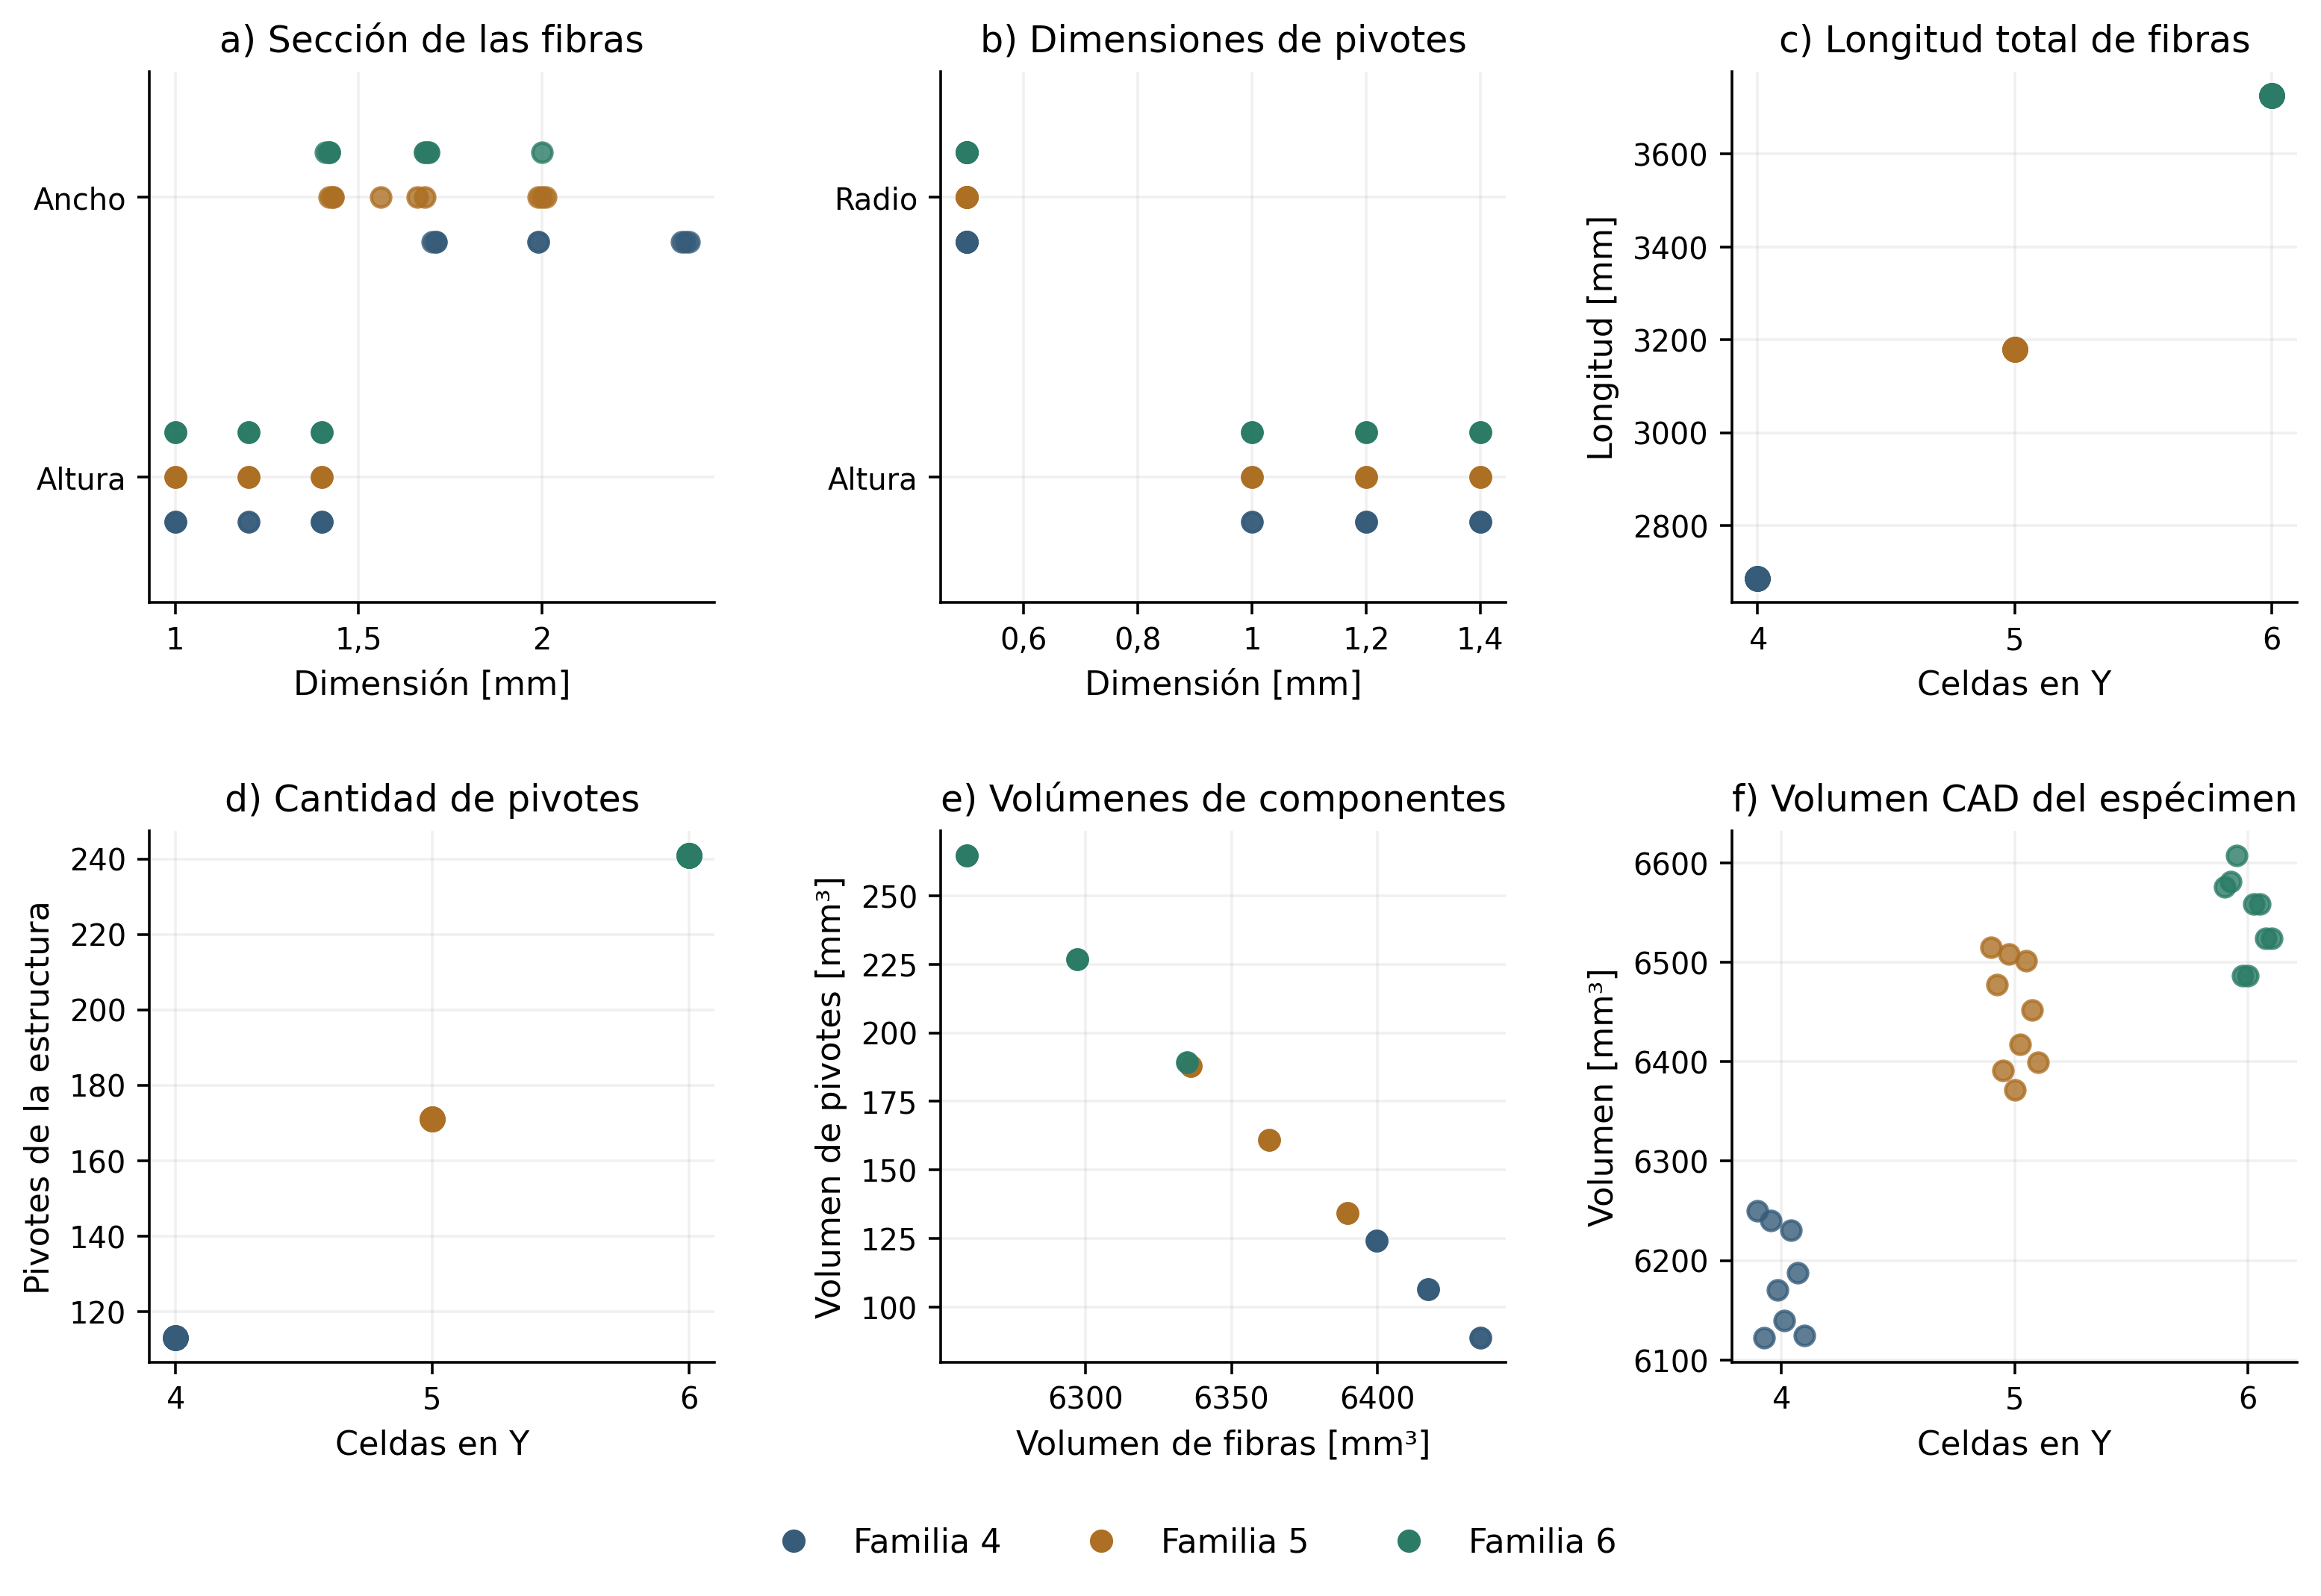
\includegraphics[width=\linewidth]{figures/EDA_geometria.png}
\caption{Caracterización de las entradas geométricas. Las posiciones corresponden a valores declarados; los colores identifican familias. Los paneles distinguen dimensiones locales, arquitectura y volúmenes. Fuente: tabla analítica y perfil univariado existente.}
\label{fig:eda-geometria}
\end{figure}

\subsection{Distribución de la carga de primera falla}
La curva acumulada muestra la fracción de respuestas inferior a cada fuerza; las cajas permiten comparar familias (Figura~\ref{fig:eda-objetivo}). La variable objetivo sigue siendo continua.

\begin{figure}[htbp]
\centering
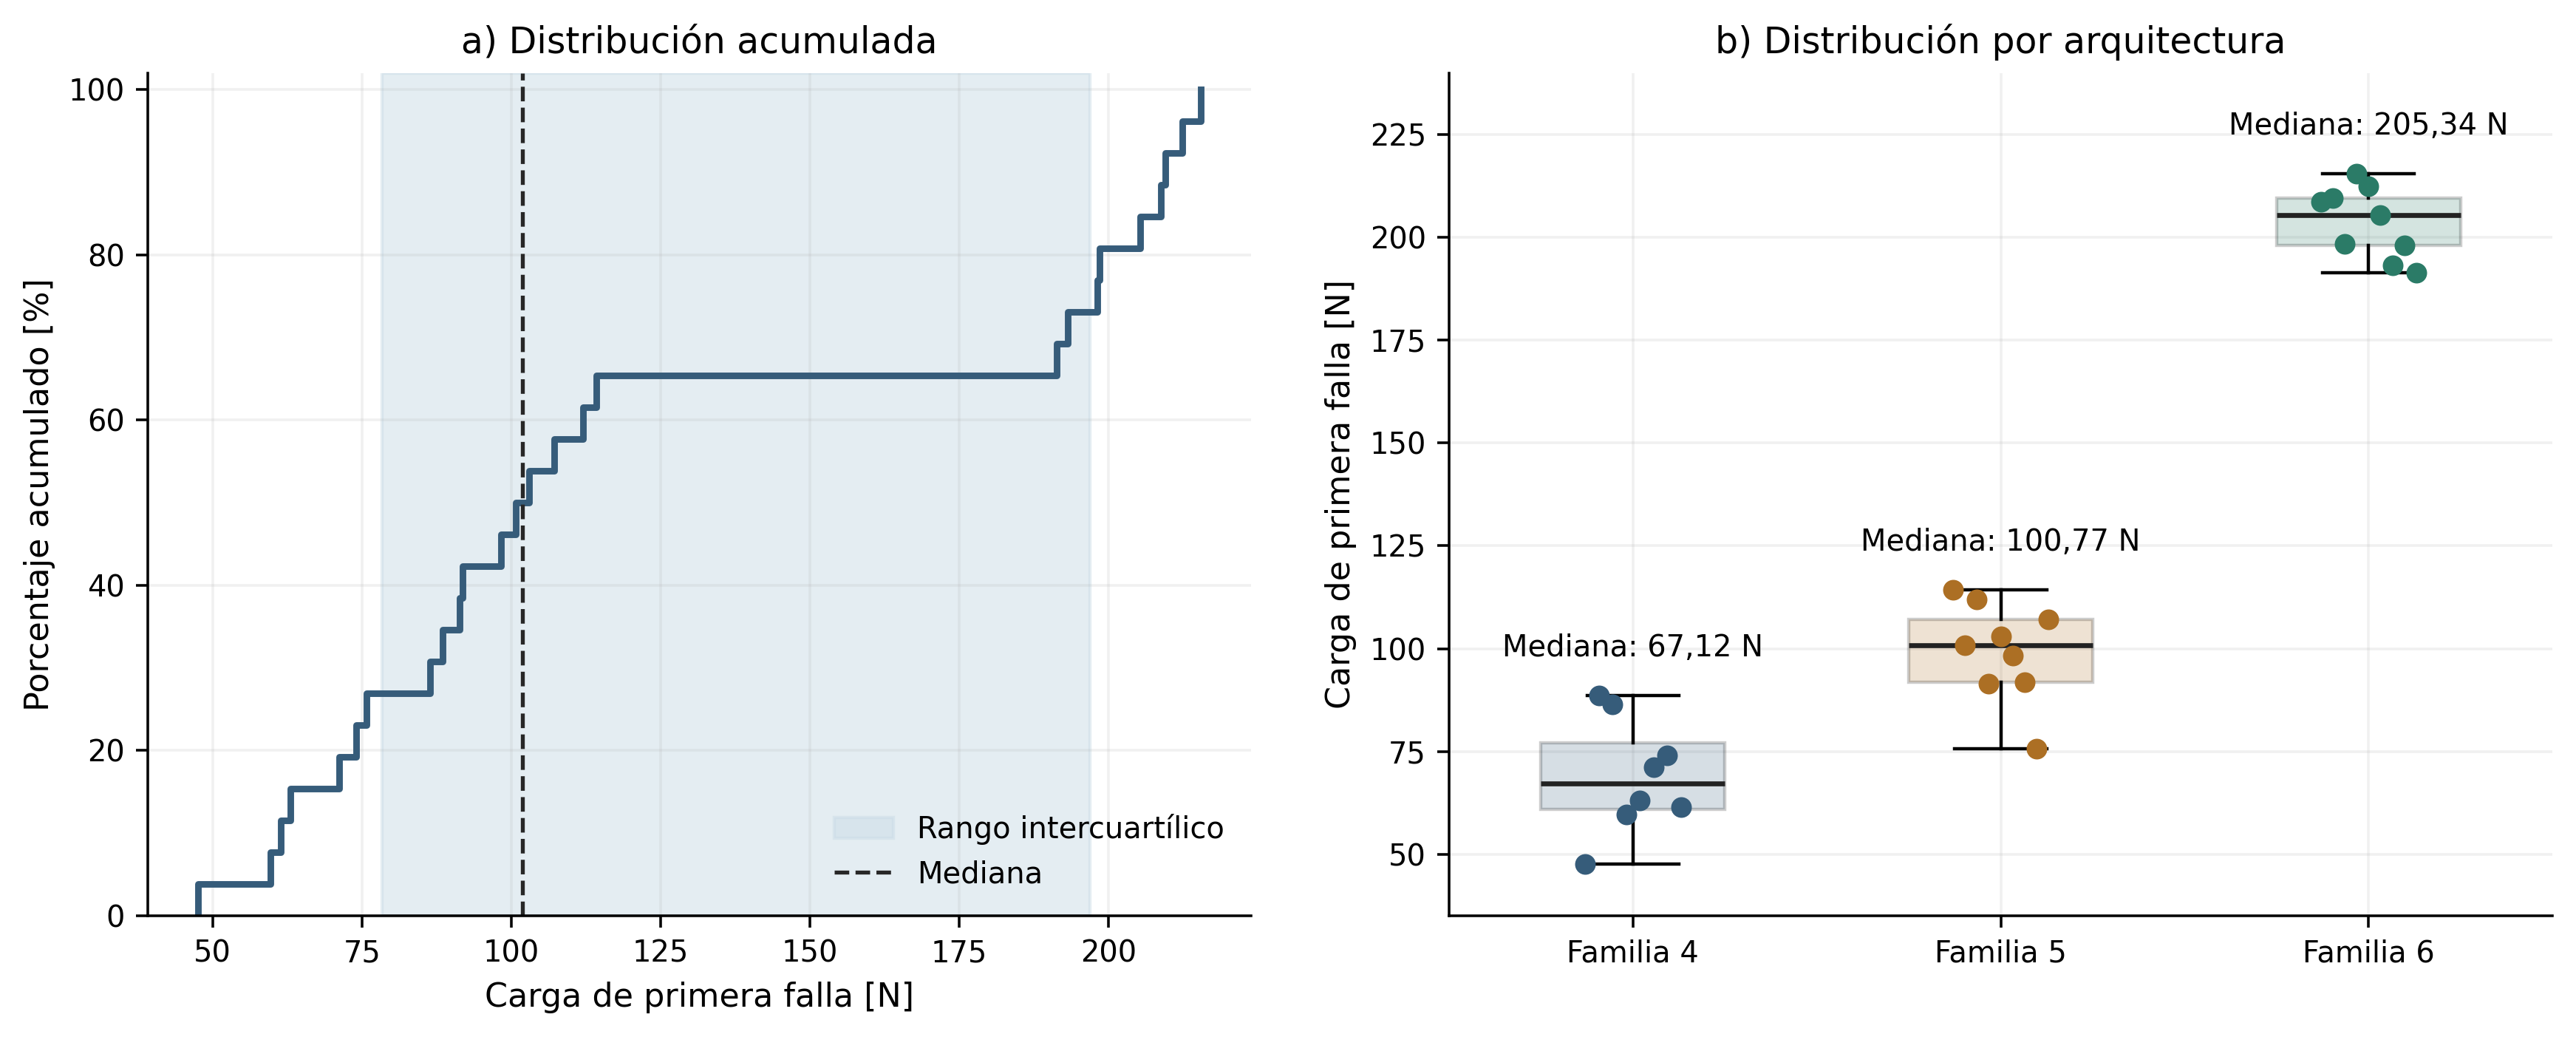
\includegraphics[width=\linewidth]{figures/EDA_primera_falla.png}
\caption{Distribución global de primera falla y comparación por familia. El intervalo sombreado delimita los cuartiles; las cajas y puntos muestran la distribución condicionada por arquitectura. No son predicciones del modelo.}
\label{fig:eda-objetivo}
\end{figure}

\begin{table}[htbp]
\centering\small\setstretch{1.0}
\caption{Resultados univariados y diferencias entre familias.}
\label{tab:eda-univariado}
\begin{tabularx}{\linewidth}{@{}p{0.19\linewidth}p{0.40\linewidth}Y@{}}
\toprule
\rowcolor{TablaCabecera} Variable & Hallazgo & Lectura \\
\midrule
Dimensiones locales & Alturas de fibra y pivote: 1--1,4~mm; ancho: 1,41--2,40~mm; radio: 0,5~mm constante. & El radio no distingue diseños observados; su relevancia mecánica fuera de esta campaña no se descarta. \\
\addlinespace
Arquitectura & Longitud: 2685,82; 3178,56; 3725,65~mm. Pivotes: 113; 171; 241, respectivamente para familias 4, 5 y 6. & Longitud y conectores varían con la familia, sin exploración independiente. \\
\addlinespace
Volúmenes de componentes & Fibras: 6259,11--6435,30~mm$^3$, CV 0,91\%. Pivotes: 88,71--264,90~mm$^3$, CV 33,79\%. Desviación estándar común: 57,68~mm$^3$. & El distinto CV refleja escalas centrales diferentes, no importancia predictiva. \\
\addlinespace
Balance de volumen & $V_f+V_p=6524{,}01$~mm$^3$ constante; CAD: 6122,21--6607,73~mm$^3$. & Componentes complementarios; CAD conserva una definición separada. \\
\addlinespace
Carga de primera falla & Rango: 47,55--215,52~N; mediana: 101,89~N; media: 126,12~N; rango intercuartílico: 118,49~N. & Centro y dispersión deben describirse conjuntamente. \\
\addlinespace
Carga por familia & Medianas 4/5/6: 67,12/100,77/205,34~N. Variación entre familias: 96,55\%; interna: 3,45\%. & Familias 4 y 5 se superponen parcialmente; 6 se separa. Es asociación descriptiva, no causalidad ni precisión predictiva. \\
\bottomrule
\end{tabularx}
\end{table}

\subsection{Análisis bivariado: entradas y primera falla}
Se recuperan Pearson (asociación lineal) y Spearman (rangos) del notebook 02. La comparación global y condicionada distingue diferencias entre familias de asociaciones internas (Figura~\ref{fig:eda-asociaciones} y Tabla~\ref{tab:eda-bivariado}).

\begin{figure}[htbp]
\centering
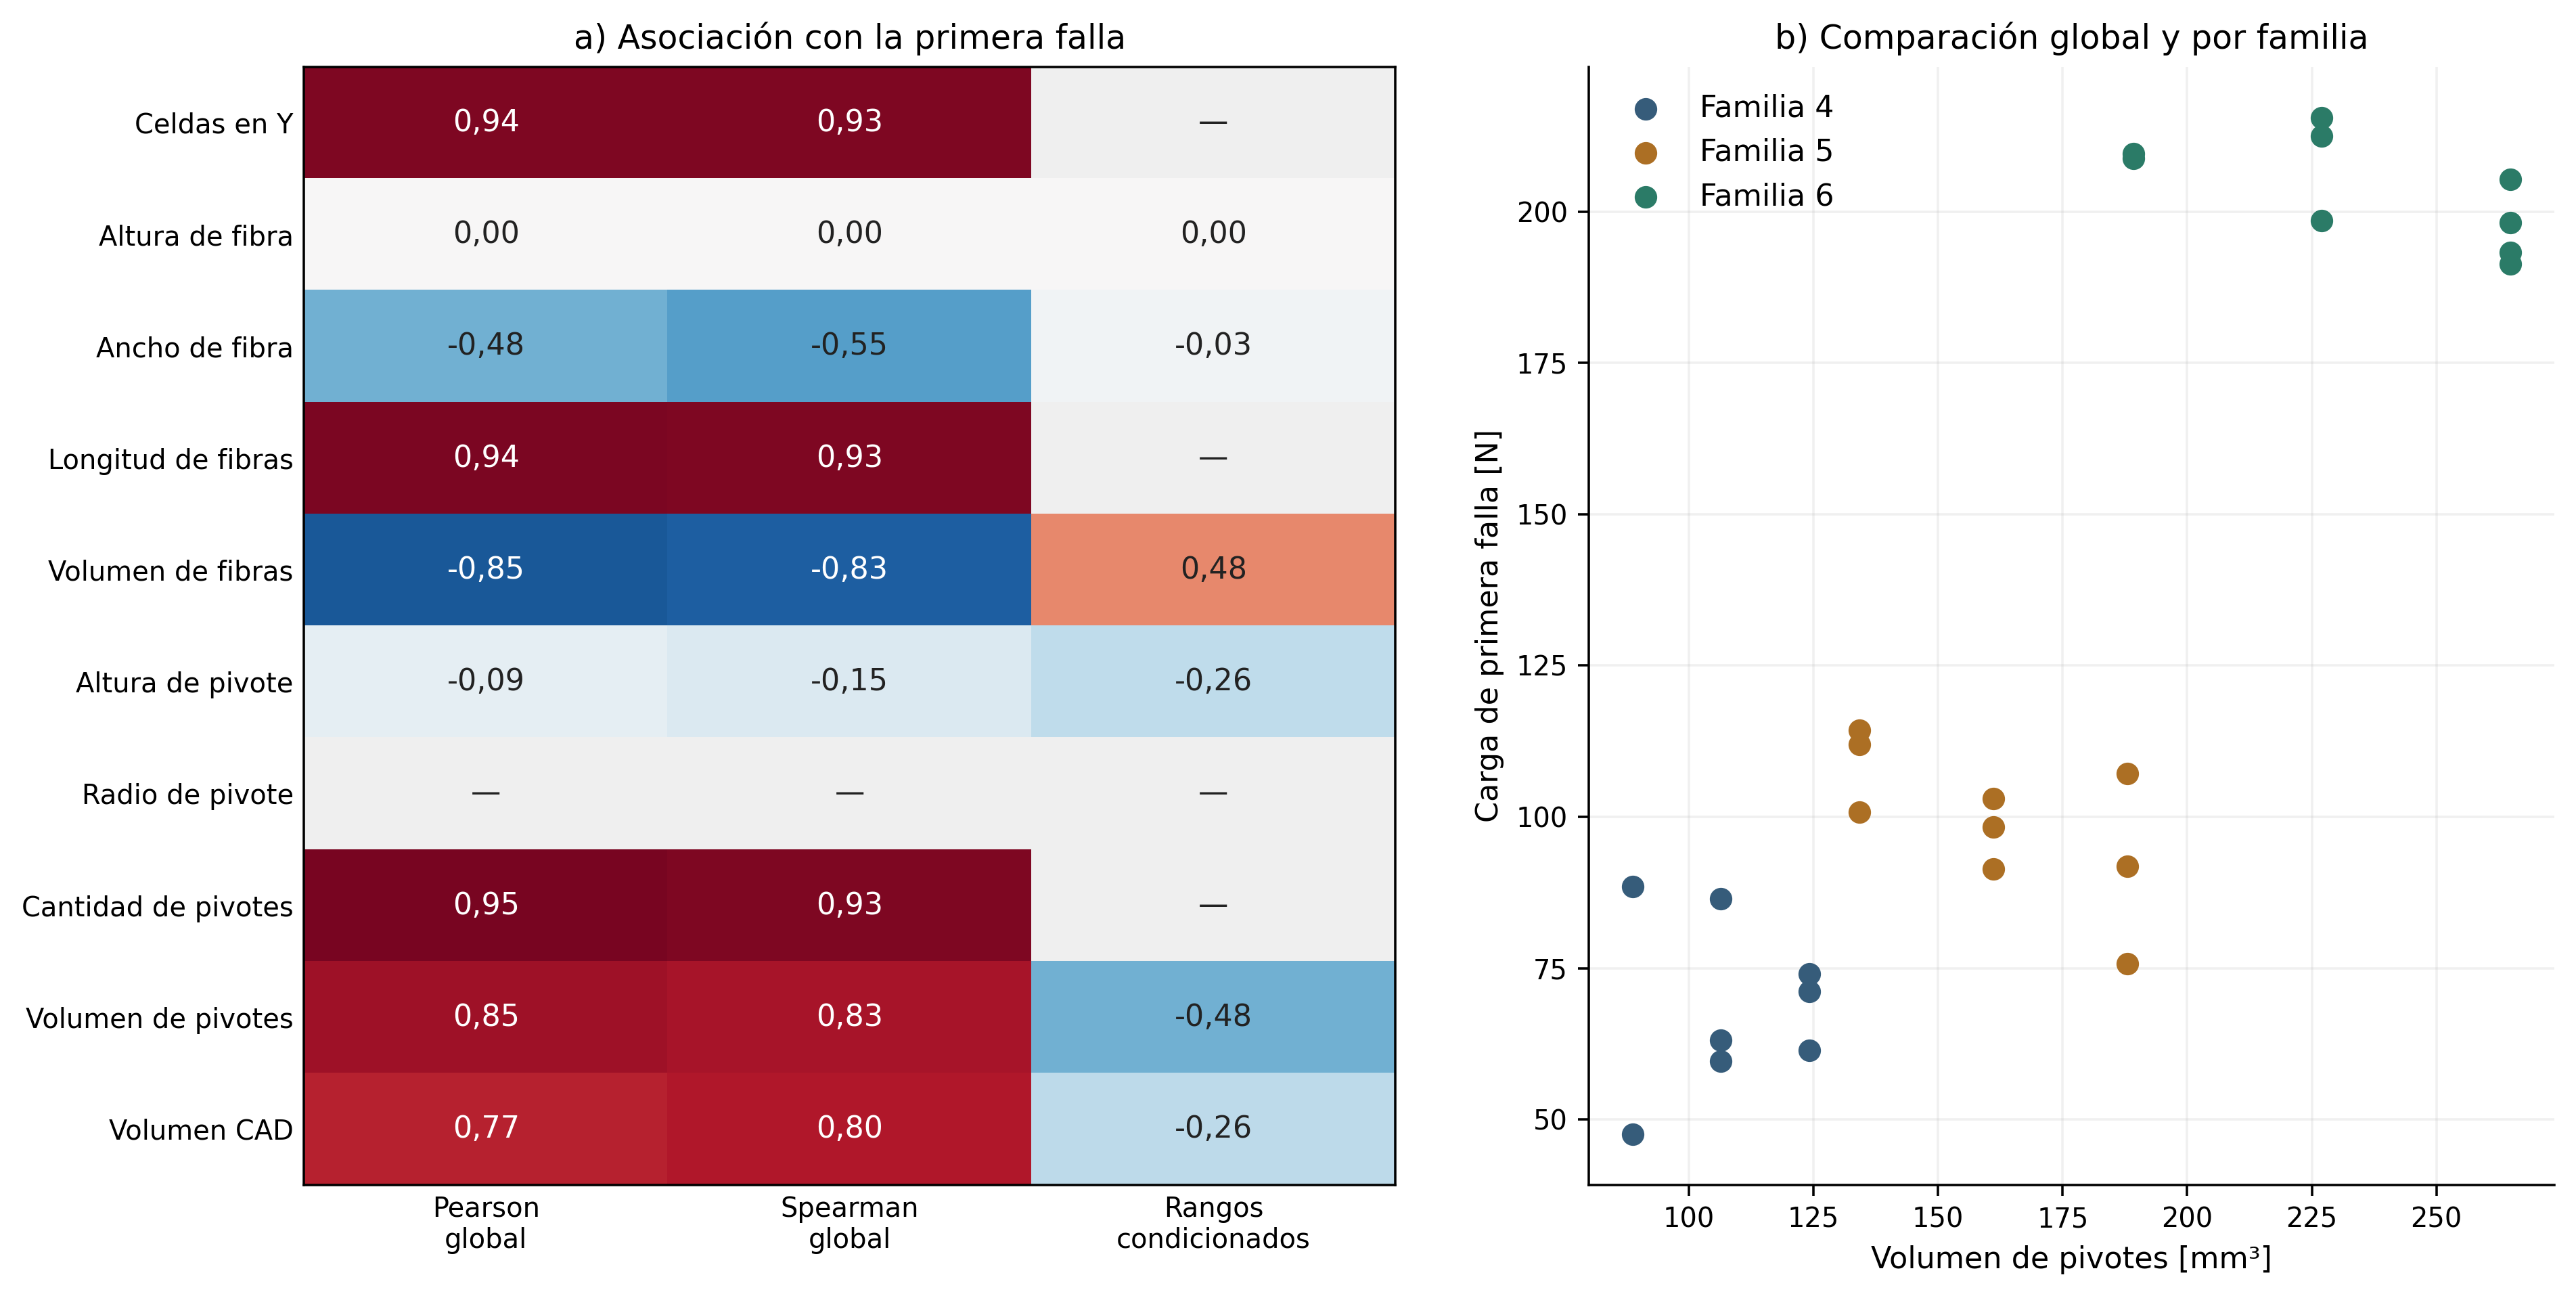
\includegraphics[width=\linewidth]{figures/EDA_asociaciones.png}
\caption{Asociaciones con la primera falla. Rangos condicionados: se resta la media de los rangos globales dentro de cada familia y se correlacionan los residuos. El guion indica un coeficiente no identificable por falta de variación; no significa cero. Fuente: tablas de asociaciones globales y condicionadas.}
\label{fig:eda-asociaciones}
\end{figure}

\begin{table}[htbp]
\centering\small\setstretch{1.0}
\caption{Asociación de las entradas con la carga de primera falla.}
\label{tab:eda-bivariado}
\begin{tabularx}{\linewidth}{@{}p{0.25\linewidth}p{0.13\linewidth}p{0.16\linewidth}Y@{}}
\toprule
\rowcolor{TablaCabecera} Variable & $\rho$ global & $\rho$ condicionado & Lectura \\
\midrule
Celdas Y, longitud y cantidad de pivotes & 0,931 & --- & Ordenan las mismas familias: no son evidencias independientes. Para celdas Y, Pearson $r=0{,}936$. \\
\addlinespace
Ancho de fibra & $-0,552$ & $-0,034$ & La asociación global se atenúa al separar familias. \\
\addlinespace
Altura de fibra & 0,000 & $\approx0$ & Asociación marginal débil; no descarta interacciones. \\
\addlinespace
Volumen de pivotes & 0,828 & $-0,477$ & Cambia de signo: el agregado no representa el efecto de aumentar volumen a arquitectura fija. \\
\addlinespace
Volumen CAD & 0,799 & $-0,265$ & También cambia de signo; debe interpretarse por familia. \\
\addlinespace
Radio de pivote & --- & --- & Constante; el coeficiente no es calculable, no equivale a cero. \\
\bottomrule
\end{tabularx}
\end{table}

Para los volúmenes complementarios, $q_{\mathrm{BH}}=0{,}0624>0{,}05$: la asociación condicionada es exploratoria. Proponer una razón logarítmica requiere comprobar su efecto sobre el error; la correlación no garantiza mejora.

\subsection{Dependencias entre variables y dimensión efectiva}
La geometría centrada tiene rango siete entre nueve columnas no constantes. El PCA estandarizado acumula 65,98\%, 83,75\% y 95,59\% de varianza en una, dos y tres componentes: describe geometría, no el objetivo ni un $R^2$. No se incorporó PCA al pipeline; las dependencias aconsejan interpretar conjuntamente las entradas y contrastar A, B y C mediante errores reservados.

\subsection{Valores atípicos, influencia y coherencia geométrica}
IQR y MAD no marcaron atípicos en geometría variable ni en primera falla. Esto no certifica normalidad ni calidad experimental; las puntuaciones que dividen por dispersión son incalculables para constantes.

\begin{figure}[htbp]
\centering
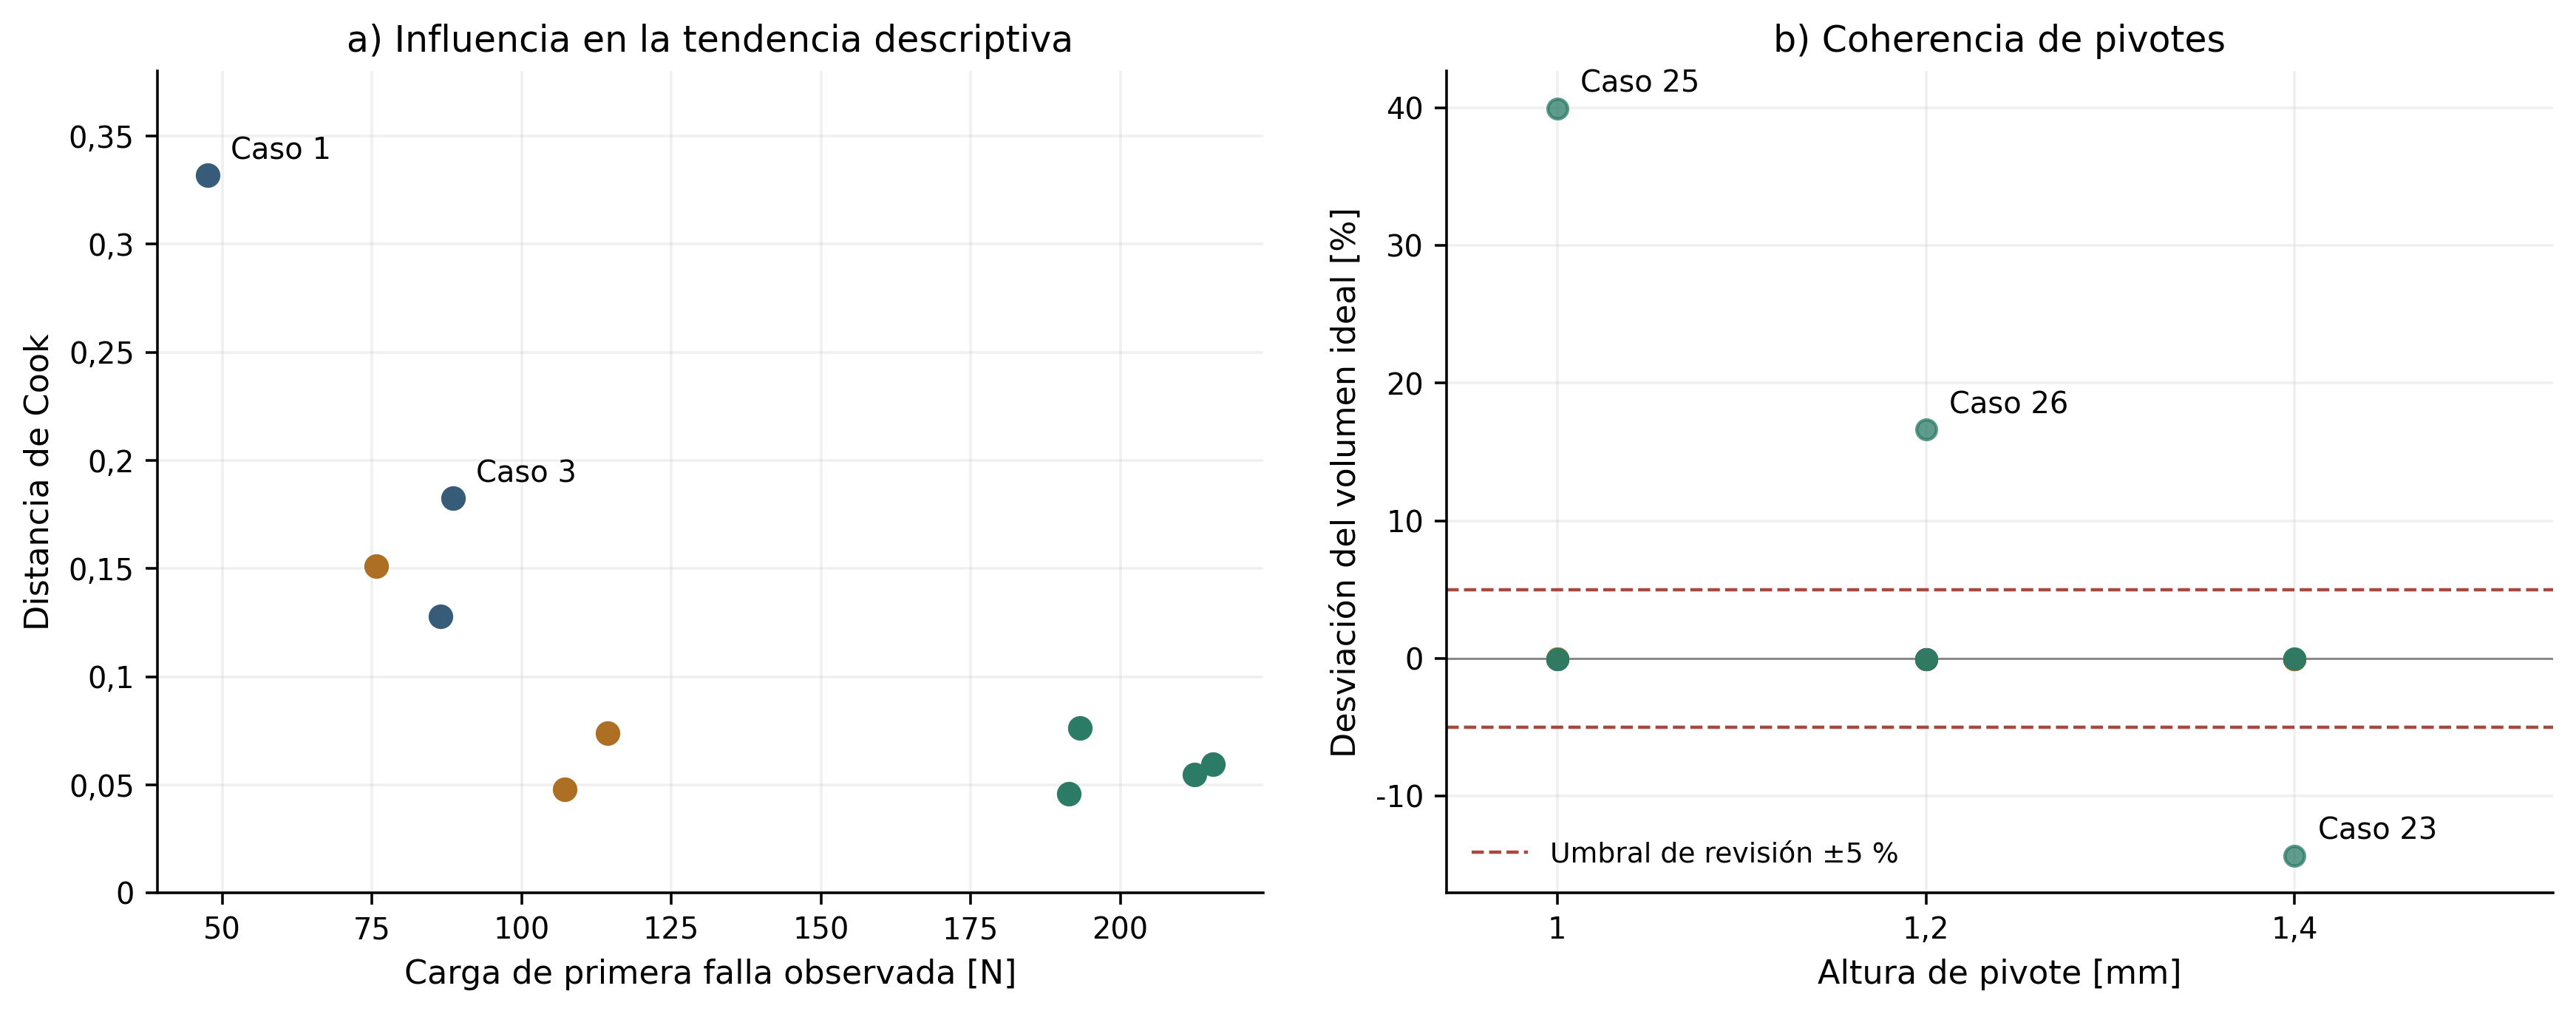
\includegraphics[width=\linewidth]{figures/EDA_influencia.png}
\caption{Diagnósticos complementarios. Izquierda: casos exportados con mayor influencia en la tendencia OLS descriptiva; Cook mide sensibilidad del ajuste, no rareza univariada. Derecha: discrepancia del volumen de pivotes respecto a cilindros ideales; el umbral de 5\% es de revisión, no tolerancia metrológica. Las etiquetas identifican casos.}
\label{fig:eda-influencia}
\end{figure}

Cook identifica influencia OLS en los casos 1 (0,332) y 3 (0,183), sin acreditar error de medición ni medir Ridge. La aproximación $V_p\approx N_p\pi r_p^2h_p$ señala discrepancias en los casos 23, 25 y 26; modela cilindros ideales y no reemplaza volúmenes declarados. Estas incidencias requieren conciliación geométrica antes de interpretar la característica derivada. Se conservaron observaciones y extremos, sin depuración orientada a mejorar métricas.

\subsection{Síntesis: del EDA a las características}
La Tabla~\ref{tab:puente-fe} conecta la evidencia con A y las variantes B y C. Las derivadas utilizan geometría previa al ensayo, sin incorporar el objetivo; su propuesta sí se apoyó en el EDA completo, por lo que la comparación sigue siendo exploratoria \cite{cawley2010}.

\begin{table}[htbp]
\centering\small\setstretch{1.0}
\caption{Del hallazgo exploratorio a las representaciones A, B y C.}
\label{tab:puente-fe}
\begin{tabularx}{\linewidth}{@{}YYY@{}}
\toprule
Hallazgo y evidencia & Interpretación & Decisión para el experimento \\
\midrule
Escalas heterogéneas y radio de 0,5~mm constante & La magnitud numérica influye en la regularización; una constante no distingue geometrías. & A: entradas originales, filtro de constantes y escalamiento dentro de entrenamiento. \\
\addlinespace
Ancho y altura de fibra combinables; momentos con asociación condicionada próxima a cero & La hipótesis es una representación geométrica no lineal, no una alta correlación individual. & B: añadir conjuntamente $bh^3/12$ y $hb^3/12$; comparar con A. \\
\addlinespace
$V_f+V_p$ constante; log-razón con $\rho$ global 0,828 y condicionado $-0,477$ & Relación dependiente de la arquitectura; representar proporción no garantiza mejora. & C: añadir $\ln(V_p/V_f)$ a B; comparar el incremento con B. \\
\addlinespace
Separación de cargas entre familias y coincidencia de factores & El agregado global puede ocultar diferencias dentro de familia. & Mantener el mismo agrupamiento en A--C y revisar error por arquitectura. \\
\addlinespace
Sin banderas IQR/MAD, pero con influencia OLS e incidencias geométricas & Ausencia de extremos univariados no asegura estabilidad del ajuste. & Conservar casos; evaluar errores individuales sin depurar observaciones para mejorar métricas. \\
\bottomrule
\end{tabularx}
\par\smallskip\small Fuente: análisis exploratorio y transformaciones de los cuadernos 02--03. Las propuestas son hipótesis que deben contrastarse con predicciones reservadas.
\end{table}


\FloatBarrier
